%
% section 6.2.3
%

\subsection{Υπηρεσία Παγκόσμιου Ιστού WWW}

Η πιο γνωστή και διαδεδομένη υπηρεσία του Διαδικτύου, είναι ο Παγκόσμιος Ιστός ή World Wide Web (www). Είναι τόσο διαδεδομένη που ο περισσότερος κόσμος τη συγχέει με την ίδια την έννοια του Διαδικτύου. Ωστόσο αυτό είναι λάθος: ο Παγκόσμιος Ιστός είναι απλά μια υπηρεσία που χρησιμοποιεί το Διαδίκτυο για να μεταφέρει τις πληροφορίες της. Ο Παγκόσμιος Ιστός είναι ένα είδος διαμορφωμένης πληροφορίας που χτίζεται πάνω από το Διαδίκτυο.

Ένα γνώρισμα του Παγκόσμιου Ιστού είναι η μη γραμμική οργάνωση της πληροφορίας του, όπως περίπου συμβαίνει σε ένα λεξικό: όταν ψάχνουμε μια λέξη δεν παίρνουμε το λεξικό από την αρχή, αλλά βρίσκουμε πρώτα το γράμμα και μετά μια κοντινή λέξη και ακολουθούμε τις λέξεις μέχρι τη σωστή.

Στον παγκόσμιο ιστό, ορίζονται οι έννοιες του \emph{υπερκειμένου} και του \emph{υπερμέσου}:

\begin{itemize}
\item \textbf{Υπερκείμενο (hypertext):} Είναι το κείμενο όπου  η πληροφορία δεν είναι οργανωμένη με γραμμική μορφή, η αναζήτηση της δε γίνεται με κάποια συγκεκριμένη σειρά, αλλά με τυχαία, ακολουθώντας τους συνδέσμους που υπάρχουν στο σώμα του κειμένου.
\item \textbf{Υπερμέσα (hypermedia):} Μια συλλογή πολυμεσικών στοιχείων (εικόνα, ήχος, βίντεο, κινούμενα σχέδια, animation) οργανωμένη με μη γραμμικό τρόπο.
\end{itemize}

Ο παγκόσμιος ιστός χρησιμοποιεί το πρωτόκολλο \emph{HTTP (Hyper Text Transfer Pro\-to\-col)} για να μεταφέρει δεδομένα. Όπως φαντάζεστε, όπως και τα υπόλοιπα πρωτόκολλα στο επίπεδο εφαρμογής, το HTTP διαθέτει κάποιες απλές εντολές στα Αγγλικά με τις οποίες ο πελάτης επικοινωνεί με τον εξυπηρετητή και ζητά στοιχεία.

\begin{figure}[!ht]
 \centering
 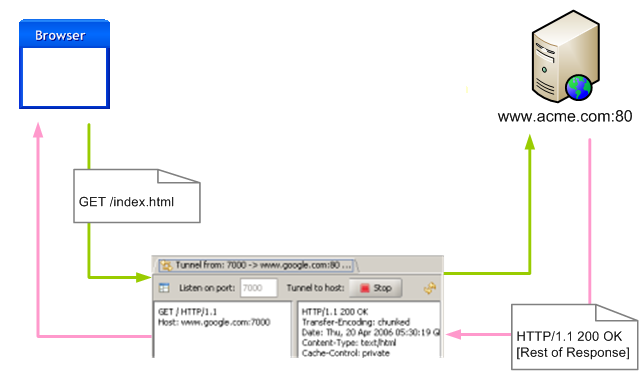
\includegraphics[width=0.95\textwidth]{images/chapter6/6-11}
 \caption {\textsl{Επικοινωνία HTTP}}
 \label{6-11}
\end{figure}

Το ρόλο του εξυπηρετητή αναλαμβάνουν προγράμματα γνωστά ως \emph{web servers}. Ένα από τα πλέον γνωστά είναι ο \emph{Apache Web Server}. Οι πληροφορίες είναι οργανωμένες σε μορφή ιστοσελίδων (web pages) και κάθε μια αντιστοιχεί σε ένα αρχείο HTML στο δίσκο του διακομιστή. Οι ιστοσελίδες είναι μια εφαρμογή υπερμέσων (περιέχουν εικόνες, κείμενο, video κλπ). Για να προσπελάσουμε μια ιστοσελίδα πρέπει να ξέρουμε τη διεύθυνση της, γνωστή και ως \emph{URL, Uniform Resource Locator}. Το URL εκτός από το όνομα αρχείου, περιέχει και την πλήρη διαδρομή που χρειαζόμαστε για να εντοπίσουμε τη σελίδα (τον εξυπηρετητή και το φάκελο στον οποίο βρίσκεται το αρχείο).

Ας πάρουμε για παράδειγμα τη σελίδα \textbf{http://www.ntua.gr/info/studies.html}. Μπορούμε να την αναλύσουμε στα παρακάτω στοιχεία:

\begin{itemize}
\item \textbf{http:} Είναι το πρωτόκολλο της υπηρεσίας που ανήκει η ιστοσελίδα. Αν είναι ``https'' πρόκειται για ασφαλή σύνδεση http
\item \textbf{www:} Δηλώνει ότι πρόκειται για σελίδα του ιστού. Μπορεί σε κάποιες περιπτώσεις να παραλείπεται
\item \textbf{ntua.gr:} Είναι η διεύθυνση του εξυπηρετητή ιστοσελίδων. Το κομμάτι αυτό όπως μπορείτε να αναγνωρίσετε είναι μια περιοχή 2ου επιπέδου, που ουσιαστικά αναφέρεται στην διεύθυνση IP του εξυπηρετητή και αναλύεται μέσω DNS
\item \textbf{/info/:} Αναφέρεται σε ένα φάκελο (κατάλογο ή directory) στο web server
\item \textbf{studies.html:} Είναι το αρχείο που περιέχει την ιστοσελίδα που θέλουμε να προσπελάσουμε
\end{itemize}

Οι ιστοσελίδες περιέχουν \emph{σημεία σύνδεσης ή hyperlinks} τα οποία μπορεί να είναι κείμενο, εικόνα κλπ. Ένα σημείο σύνδεσης μπορεί να παραπέμπει:

\begin{itemize}
\item Σε άλλο σημείο πάνω στην ίδια σελίδα (anchor)
\item Σε άλλη ιστοσελίδα στον ίδιο εξυπηρετητή / site (εσωτερικός σύνδεσμος)
\item Σε άλλη ιστοσελίδα άλλου εξυπηρετητή / διαφορετικού site οπουδήποτε στο Διαδίκτυο (εξωτερικός σύνδεσμος)
\end{itemize}

Η ίδια η ιστοσελίδα δεν ακολουθεί τις συμβάσεις των έντυπων βιβλίων (συγκεκριμένο μέγεθος για εκτύπωση σε χαρτί) αλλά μπορεί να έχει μεγαλύτερο μήκος και πλάτος από ότι εμφανίζεται στην οθόνη (εξάλλου, διαφορετικές οθόνες έχουν διαφορετική ανάλυση και ειδικά σε φορητές συσκευές υπάρχει μεγάλη διακύμανση).

Ένα σύνολο πληροφοριών που οργανώνεται σε μορφή ιστοσελίδων ονομάζεται \emph{τοποθεσία (site)}.

Οι \emph{Φυλλομετρητές (browsers)} είναι το πρόγραμμα πελάτης που χρησιμοποιεί ο χρήστης για να απευθύνει αιτήματα στο Web Server. Υπάρχουν πολλά προγράμματα φυλλομετρητών για διάφορα λειτουργικά συστήματα: Firefox, Chrome, Opera, Edge κλπ. Οι βασικές λειτουργίες που συναντάμε σε ένα πρόγραμμα φυλλομετρητή, είναι:

\begin{itemize}
\item Αποστέλλει αιτήματα / ερωτήματα στους εξυπηρετητές ιστοσελίδων χρησιμοποιώντας το πρωτόκολλο HTTP
\item Σχεδιάζει την ιστοσελίδα σύμφωνα με τις πληροφορίες που του έστειλε ο εξυπηρετητής. Οι φυλλομετρητές διαθέτουν μια μηχανή απεικόνισης που ερμηνεύει τις εντολές της γλώσσας HTML και σχεδιάζει τη σελίδα στην οθόνη σύμφωνα με αυτές
\item Τονίζει τα σημεία σύνδεσης όπου υπάρχουν, ώστε να είναι ευδιάκριτα και να εντοπίζονται εύκολα από το χρήστη πάνω στη σελίδα
\item Δίνει τη δυνατότητα αποθήκευσης των ιστοσελίδων σε καταλόγους
\item Κρατάει ιστορικό με τις διευθύνσεις των ιστοσελίδων που έχουμε επισκεφθεί
\end{itemize}

Με τους φυλλομετρητές έχουμε τη δυνατότητα να διαβάζουμε ιστοσελίδες του Διαδικτύου, οι οποίες είναι στη πραγματικότητα σελίδες υπερμέσων (μπορούν να περιέχουν φωτογραφίες, ήχο, animation κλπ). Για να διαβάσουμε μια ιστοσελίδα θα πρέπει να ξέρουμε το όνομα της, το φάκελο στον οποίο είναι αποθηκευμένη και τη διεύθυνση του web server (με λίγα λόγια το URL της). Στην πραγματικότητα τα πράγματα είναι πιο απλά: τυπικά δεν χρειάζεται να θυμόμαστε τίποτα περισσότερο από τη διεύθυνση του εξυπηρετητή. Οι εξυπηρετητές είναι ρυθμισμένοι όταν δεν ζητηθεί κάποια συγκεκριμένη ιστοσελίδα να δίνουν μια \emph{αρχική προεπιλεγμένη σελίδα (default page)}. Συνήθως αντιστοιχεί στο αρχείο index.html ή index.htm ή default.html. Μέσα από τους συνδέσμους που υπάρχουν σε αυτή τη σελίδα μπορούμε να αναζητήσουμε τις πληροφορίες που θέλουμε αλλά και να πλοηγηθούμε στις υπόλοιπες σελίδες του site.
